\section{紧自伴算子的谱分解}
\label{sec:ospec-compact-self-adjoint}

实对称矩阵有一组由特征向量组成的标准正交基，矩阵在这组基下是实对角矩阵。上一节的累积积分说明，紧性本身不足以给出这种结构；对角算子$A(x_n)=(x_n/n)$却正好具备它：特征向量$e_n$组成标准正交基，算子就是沿每个基方向乘以一个数。二者的差别在于$A$是自伴的。本节证明，在Hilbert空间中对紧算子再加入自伴条件，就得到实特征值、正交的特征方向，以及Hilbert范数下的特征展开。

本节设$H$是实或复Hilbert空间，$T\in\mathcal B(H)$紧且自伴，即$\langle v,Tu\rangle=\langle Tv,u\rangle$对一切$u,v$成立。证明不需要复化：自伴算子的特征值将被证明是实数。

\begin{theorem}[紧自伴算子的谱分解]
\label{thm:ospec-compact-self-adjoint}
设$T$是Hilbert空间$H$上的紧自伴算子。则：
\begin{enumerate}
\item $T$的特征值都是实数，属于不同特征值的特征向量互相正交；
\item 每个非零特征值的特征空间有限维；对每个$\delta>0$，满足$\lvert\lambda\rvert\geq\delta$的特征值只有有限个；
\item 存在有限或可数的标准正交序列$(e_j)$及非零实数$\lambda_j$（按重数重复列出，$\lvert\lambda_1\rvert\geq\lvert\lambda_2\rvert\geq\cdots$，序列无限时$\lambda_j\to0$），使$Te_j=\lambda_je_j$，$(e_j)$的闭张成等于$(\ker T)^\perp$，并且对每个$u\in H$，
\begin{equation}
u=u_0+\sum_j\langle e_j,u\rangle e_j,\qquad Tu=\sum_j\lambda_j\langle e_j,u\rangle e_j,\qquad u_0\in\ker T,
\label{eq:ospec-spectral-expansion}
\end{equation}
两个级数都按$H$的范数收敛。
\end{enumerate}
\end{theorem}

证明的主线是：先说明自伴算子的范数可以由二次型$\langle u,Tu\rangle$读出，再用紧性找到使二次型绝对值最大的方向，它就是一个特征方向；然后把算子限制到这个方向的正交补上，重复同样的步骤。下面分步完成。

\paragraph{特征值与正交性}
设$Tu=\lambda u$，$u\neq0$。由内积对第一个变量共轭线性，$\langle u,Tu\rangle=\lambda\lVert u\rVert^2$，$\langle Tu,u\rangle=\bar\lambda\lVert u\rVert^2$；自伴使两者相等，所以$\lambda=\bar\lambda$是实数。再设$Tv=\mu v$，$\mu\neq\lambda$，两者都是实数，于是
\[
\lambda\langle v,u\rangle=\langle v,Tu\rangle=\langle Tv,u\rangle=\mu\langle v,u\rangle ,
\]
从而$\langle v,u\rangle=0$。这证明了结论1。

\paragraph{非零特征值的有限性}
设$(e_j)$是一列两两正交的单位特征向量，$Te_j=\lambda_je_j$且$\lvert\lambda_j\rvert\geq\delta>0$；它们可以来自同一个特征空间的标准正交组，也可以属于不同特征值（由结论1自动正交）。对$j\neq k$，
\[
\lVert Te_j-Te_k\rVert^2=\lVert\lambda_je_j-\lambda_ke_k\rVert^2=\lvert\lambda_j\rvert^2+\lvert\lambda_k\rvert^2\geq2\delta^2 ,
\]
输出列没有柯西子列，与紧性矛盾，所以这种序列只能有限长。取同一特征空间中的标准正交组，即知非零特征空间有限维；取不同特征值的特征向量，即知$\lvert\lambda\rvert\geq\delta$的特征值只有有限个。这证明了结论2，它在Hilbert空间中重现了上一节定理的相应部分，而且证明更短，因为正交性代替了Riesz引理。

\paragraph{二次型给出范数}
令$M=\sup_{\lVert u\rVert=1}\lvert\langle u,Tu\rangle\rvert$。由Cauchy--Schwarz不等式$M\leq\lVert T\rVert$。反向不等式要从二次型恢复$\lVert Tu\rVert$。自伴使$\langle u,Tv\rangle=\langle Tu,v\rangle=\overline{\langle v,Tu\rangle}$，展开可得
\[
\langle u+v,T(u+v)\rangle-\langle u-v,T(u-v)\rangle=2\langle u,Tv\rangle+2\langle v,Tu\rangle=4\operatorname{Re}\langle v,Tu\rangle .
\]
左边两项的绝对值分别不超过$M\lVert u+v\rVert^2$与$M\lVert u-v\rVert^2$，再用平行四边形恒等式$\lVert u+v\rVert^2+\lVert u-v\rVert^2=2\lVert u\rVert^2+2\lVert v\rVert^2$，得
\[
4\operatorname{Re}\langle v,Tu\rangle\leq2M\bigl(\lVert u\rVert^2+\lVert v\rVert^2\bigr).
\]
对单位向量$u$且$Tu\neq0$，取$v=Tu/\lVert Tu\rVert$，则$\operatorname{Re}\langle v,Tu\rangle=\lVert Tu\rVert$，上式化为$\lVert Tu\rVert\leq M$。因此$\lVert T\rVert=M$。

\paragraph{紧性给出极值方向}
设$T\neq0$。取单位向量$u_n$使$\lvert\langle u_n,Tu_n\rangle\rvert\to\lVert T\rVert$。这些二次型都是实数，可以抽出子列使它们的符号一致，于是$\langle u_n,Tu_n\rangle\to\lambda$，其中$\lambda=\lVert T\rVert$或$-\lVert T\rVert$。这里不能预先假定$\lambda$为正：自伴算子的二次型可以取负值，绝对值最大的特征值可能是负的。展开
\[
\lVert Tu_n-\lambda u_n\rVert^2=\lVert Tu_n\rVert^2-2\lambda\langle u_n,Tu_n\rangle+\lambda^2\leq2\lambda^2-2\lambda\langle u_n,Tu_n\rangle\to0 ,
\]
其中用到$\lVert Tu_n\rVert\leq\lVert T\rVert=\lvert\lambda\rvert$。

由紧性，可再抽子列使$Tu_n\to w$。于是$\lambda u_n=Tu_n-(Tu_n-\lambda u_n)\to w$，即$u_n\to e=w/\lambda$，$\lVert e\rVert=1$，并且$Te=\lim Tu_n=w=\lambda e$。所以$\pm\lVert T\rVert$中至少有一个是特征值，相应单位特征向量为$e$。

\paragraph{逐步分解与零空间}
记$e_1=e$，$\lambda_1=\lambda$。正交补$H_2=\{e_1\}^\perp$在$T$下不变：若$\langle e_1,v\rangle=0$，则$\langle e_1,Tv\rangle=\langle Te_1,v\rangle=\lambda_1\langle e_1,v\rangle=0$。$T$在$H_2$上的限制仍是紧自伴算子，范数不超过$\lVert T\rVert$。若这个限制为零，过程停止；否则重复上一段，得到$e_2\perp e_1$及$\lvert\lambda_2\rvert=\lVert T|_{H_2}\rVert\leq\lvert\lambda_1\rvert$。依此类推，在$H_k=\{e_1,\ldots,e_{k-1}\}^\perp$上取$e_k$。若过程不停止，由结论2，$\lambda_k\to0$。

令$M$为$(e_j)$的闭张成。$M^\perp$含于每个$H_k$，所以$T$在$M^\perp$上的限制的范数不超过每个$\lvert\lambda_k\rvert$；过程无限时它趋于零，有限时按停止条件本身为零。因此$T$在$M^\perp$上恒为零，$M^\perp\subseteq\ker T$。反过来，若$Tu=0$，则对每个$j$，
\[
\langle e_j,u\rangle=\frac{1}{\lambda_j}\langle Te_j,u\rangle=\frac{1}{\lambda_j}\langle e_j,Tu\rangle=0 ,
\]
所以$\ker T\subseteq M^\perp$。二者相等，$M=(M^\perp)^\perp=(\ker T)^\perp$。这也说明每个非零特征值都已出现在$(\lambda_j)$中：属于非零特征值$\mu$的特征向量与$\ker T$正交，因而落在$M$中；若$\mu$不等于任何$\lambda_j$，由结论1它与所有$e_j$正交，只能为零。

\paragraph{展开式}
$u$在闭子空间$M$上的正交投影为$\sum_j\langle e_j,u\rangle e_j$，级数按范数收敛（第~\ref{chap:inner-product-spaces}章）；余项$u_0=u-P_Mu$属于$M^\perp=\ker T$。把$T$作用于投影的部分和，由连续性得$Tu=\sum_j\lambda_j\langle e_j,u\rangle e_j$。这就是式\eqref{eq:ospec-spectral-expansion}，定理证毕。

\paragraph{空间的分解与有限谱截断}
定理把$H$分成两部分：$\ker T$与非零特征方向的闭张成$(\ker T)^\perp$。任意向量$u$的位置由它在$\ker T$中的分量$u_0$与各特征方向上的系数$\langle e_j,u\rangle$完全确定，$T$消去$u_0$，并把第$j$个系数乘以$\lambda_j$。由勾股定理，
\[
\lVert u\rVert^2=\lVert u_0\rVert^2+\sum_j\lvert\langle e_j,u\rangle\rvert^2,\qquad\lVert Tu\rVert^2=\sum_j\lambda_j^2\lvert\langle e_j,u\rangle\rvert^2 .
\]

只保留前$m$个特征方向，得到有限秩算子$T_mu=\sum_{j\leq m}\lambda_j\langle e_j,u\rangle e_j$。由上式，
\[
\lVert(T-T_m)u\rVert^2=\sum_{j>m}\lambda_j^2\lvert\langle e_j,u\rangle\rvert^2\leq\lambda_{m+1}^2\lVert u\rVert^2 ,
\]
取$u=e_{m+1}$时等号成立，所以$\lVert T-T_m\rVert=\lvert\lambda_{m+1}\rvert$（非零特征值用尽时约定为$0$）。特征值按绝对值递减排列，截断误差就是第一个被舍弃的特征值的绝对值；这给出第~\ref{chap:linear-operators}章有限秩逼近的一个具体而经济的选择。

\paragraph{贯穿例子}
回到$L^2([-1,1],\mu)$，$\mathrm d\mu=\mathrm dz/2$，核$1+xz$给出$(Tf)(x)=\int f\,\mathrm d\mu+x\int zf\,\mathrm d\mu$。核实对称，$T$紧自伴。由$T1=1$与$Tx=x\int z^2\,\mathrm d\mu=\tfrac13x$，单位特征向量为$e_1=1$、$e_2=\sqrt3\,x$，特征值$\lambda_1=1$、$\lambda_2=1/3$，于是
\[
Tf=\langle e_1,f\rangle e_1+\tfrac13\langle e_2,f\rangle e_2 .
\]
与$1,x$都正交的函数组成$\ker T$，例如$x^2-1/3$，这个零空间是无限维的。截断一项的误差为$\lVert T-T_1\rVert=1/3$。

把核换成$1-6xz$，常数方向不变，线性方向变为$Tx=-6x\int z^2\,\mathrm d\mu=-2x$，绝对值最大的特征值是$-2$。若只寻找正的最大特征值，就会漏掉这个主导方向，这正是证明中不预设$\lambda>0$的原因。图~\ref{fig:ospec-spectral-stretch}在两组特征方向的系数平面上画出了这两类伸缩。

\begin{figure}[!htb]
  \centering
  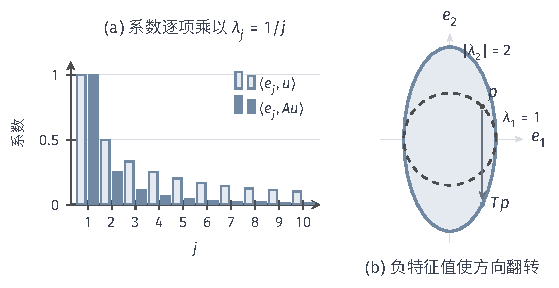
\includegraphics[width=94.6mm]{figures/02-abstract-mathematics/03-function-spaces/tikz/c3-spectral-stretch/figure.pdf}
  \caption{紧自伴算子沿特征方向逐个伸缩。(a)~$\ell^2$上$A=\operatorname{diag}(1/j)$，浅色条为$u$的系数$\langle e_j,u\rangle=1/j$，深色条为$Au$的系数$1/j^2$；(b)~$L^2([-1,1],\mathrm dz/2)$上核$1-6xz$的积分算子，在$e_1=1$、$e_2=\sqrt3x$的系数平面上把虚线单位圆映为实线椭圆：$e_1$方向乘$1$，$e_2$方向乘$-2$。与$1,x$正交的方向全部被映为零，图中未画出。}
  \label{fig:ospec-spectral-stretch}
\end{figure}

谱分解中的级数按Hilbert空间的范数收敛。对$L^2$中的函数，这意味着平方积分误差趋于零，并不意味着在每一点或一致地收敛；第~\ref{sec:ospec-integral-expansion}节在积分核上具体讨论这一区别。
